\documentclass[11pt,letterpaper]{article}

\usepackage[top=1in,bottom=1in,left=1in,right=1in]{geometry}
\usepackage{amsmath,amssymb}
\usepackage{booktabs}
\usepackage{array}
\usepackage{xcolor}
\usepackage{enumitem}
\usepackage{graphicx}
\usepackage{hyperref}
\usepackage{microtype}

\graphicspath{{../../sensitivity_analysis/figures/}{../../sensitivity_analysis/figures/robustness/}{../../../backend/syntheticData/figures/}}

\hypersetup{colorlinks=true, linkcolor=blue!70!black, urlcolor=blue!70!black}
\setlist[enumerate]{leftmargin=1.8em, itemsep=2pt, topsep=3pt}
\setlist[itemize]{leftmargin=1.5em, itemsep=2pt, topsep=3pt}

\title{\textbf{Paper A Methods: MSSD Decision Engine, Synthetic Data, Calibration and Robustness}}
\author{Tien (Tyler) Le}
\date{October 2026}

\begin{document}

\maketitle

\noindent This document merges and replaces the two earlier drafts, ``Algorithmic Calibration and Micro-Randomized Decision Engine'' and ``Synthetic Data Generation and Algorithmic Robustness''. Every simulation result reported here uses the production 1--7 Likert scale. Earlier 1--5 results are superseded.

\section{MSSD Definition and Decision Rules}

\subsection{Notation}

Throughout, $t$ is the prompt index: $t = 1, 2, \dots, n_i$ counts participant $i$'s check-in prompts in time order. It is not a day count. Day $d$ and within-day position $k$ are derived from $t$ where needed (Section 2.4).

\subsection{Mathematical Definition}

Let $x_{i,t}$ be the value that participant $i$'s Ecological Momentary Assessment (EMA) check-in at prompt $t$ contributes to the engine. In the single-item simulations of Sections 2--8, $x_{i,t} \in \{1, 2, \dots, 7\}$ is one integer Likert response. In production it is the three-item mean defined in Section 1.3, and Section 5 tests whether the single-item results carry over to it. The full-series mean square of successive differences (MSSD) is
\begin{equation}
\text{MSSD}_i = \frac{1}{n_i - 1} \sum_{t=2}^{n_i} (x_{i,t} - x_{i,t-1})^2 .
\end{equation}
A full-series value is not suited to real-time use, because it averages over earlier shifts in a participant's baseline rather than isolating recent swings. The decision engine therefore uses a rolling form over the most recent $w$ successive differences, with $w$ = 3:
\begin{equation}
\widehat{\text{MSSD}}_{i,t} = \frac{1}{\min(w,\, t - 1)} \sum_{k=\max(2,\, t - w + 1)}^{t} (x_{i,k} - x_{i,k-1})^2 .
\end{equation}
At prompts 2 and 3 the engine averages the differences available so far. How a missed prompt is treated differs between the published simulation and production. In the simulation a missed prompt is a missing row, so a difference involving it is dropped. In production a missed prompt has no row at all, so the difference spans it (Section 1.3). Offline audits should use the value logged at decision time in \texttt{JITAILog.observed\_mssd}, not a recomputed full-series MSSD, because the rolling and full-series quantities differ.

\subsection{Production MSSD Input}

The production engine input is built by \texttt{build\_decision\_frame} in \texttt{backend/app/tasks.py}. It is scored by \texttt{calculate\_mssd} and \texttt{apply\_decision\_rules} in the module \texttt{decision\_engine.py}, under \texttt{backend/decision\_engine/}. Exactly:

\begin{enumerate}
    \item \textbf{Rows.} One row per \emph{completed} check-in that contains all three of \texttt{B1\_valence}, \texttt{B2\_stress} and \texttt{B1\_arousal}, in order of the time the check-in was served. Scheduled, outcome and extra check-ins all count. A check-in missing any of the three items, such as a feedback-only check-in, contributes no row. Missed prompts produce no row.
    \item \textbf{Value.} The row's value is the unweighted mean of the three raw item scores (1--7 each):
    \begin{equation}
    y_{i,j} = \tfrac{1}{3}\left(V_{i,j} + S_{i,j} + A_{i,j}\right),
    \end{equation}
    where $j$ indexes participant $i$'s completed check-ins, not prompts. No item is reverse-coded. Valence is scored high = positive and stress high = negative, so opposite movements in the two partly cancel. The value lies on a grid of thirds (1, 4/3, \dots, 7) rather than on the integers.
    \item \textbf{Differences.} The rolling MSSD of Section 1.2 is applied to $y_{i,j}$ with $j$ in place of $t$:
    \begin{equation}
    \widehat{\text{MSSD}}_{i,j} = \frac{1}{\min(3,\, j - 1)} \sum_{k=\max(2,\, j - 2)}^{j} (y_{i,k} - y_{i,k-1})^2 .
    \end{equation}
    Because consecutive rows are consecutive \emph{completed} check-ins, a difference spans any missed prompts between them. Differences also \textbf{cross the overnight gap}: the first check-in of a day is differenced against the last check-in of the previous day, and nothing in the engine marks or down-weights that difference.
    \item \textbf{Threshold and gate.} As in Section 1.4: the expanding 80th percentile of the participant's earlier values of $\widehat{\text{MSSD}}_{i,j}$, available once three earlier values exist, with a strict $>$ gate.
\end{enumerate}

Section 9 replays this construction from the stored item responses for the Phase 1 participants. The replay reproduces the logged \texttt{observed\_mssd} and \texttt{threshold\_at\_decision} on all 524 engine-logged decisions, so the description above is the code, not an approximation of it.

The unreversed mean is the mapping confirmed with the PI on 2026-08-17. Whether stress should be reverse-coded before averaging is a design question for the PI, not a change made here. Section 5 shows that the threshold-crossing rate and dosage are insensitive to the valence--stress correlation, because the threshold is relative to each participant's own history. The choice changes which moments count as volatile, not how many.

\subsection{Decision Pipeline}

At each completed check-in the production engine applies the following gates in order. A decision point that fails a gate is logged with its reason and is not randomized.

\begin{enumerate}
    \item \textbf{Run-in.} Per the protocol, the first seven days after enrollment are a run-in. Check-ins are collected and the threshold history accrues, but no decision point is randomized (\texttt{RUN\_IN\_DAYS} = 7).
    \item \textbf{Distress override.} An active baseline or momentary distress flag suspends randomization for that participant, and the app shows a resource card instead (protocol Section 11).
    \item \textbf{Minimum history.} The threshold below needs at least three earlier rolling MSSD values. Prompt 1 has no difference, and prompts 2--4 produce MSSD values but cannot yet be compared with a threshold. The earliest prompt that can be eligible is therefore prompt 5. This is a property of the prompt sequence and is separate from the seven-day run-in.
    \item \textbf{Within-person threshold.} The cutoff is the 80th percentile of the participant's own earlier rolling MSSD values:
    \begin{equation}
    \Theta_{i,t} = \text{Quantile}_{0.80}\left(\{\widehat{\text{MSSD}}_{i,1}, \dots, \widehat{\text{MSSD}}_{i,t-1}\}\right).
    \end{equation}
    The current prompt is excluded, so it cannot raise its own bar. The window is expanding: every earlier value is kept.
    \item \textbf{MSSD gate.} A decision point passes when $\widehat{\text{MSSD}}_{i,t} > \Theta_{i,t}$. A value equal to the threshold does not pass. The gate responds to volatility relative to the participant's own history, not to the level of any response.
    \item \textbf{Cooldown.} No prompt is sent within 60 minutes of a prompt already sent.
    \item \textbf{Daily cap.} No more than 4 prompts are sent per participant per calendar day.
    \item \textbf{Micro-randomization.} A decision point that passes every gate above is \emph{available}. It is randomized to send with probability 0.5:
    \begin{equation}
    A_{i,t} \sim \text{Bernoulli}(p), \qquad p = 0.5 .
    \end{equation}
\end{enumerate}

The simulation engine (\texttt{apply\_decision\_rules}) implements gates 3--7 only. Section 3 lists the differences.

\section{Synthetic Data Generation}

\subsection{Generative Process}

Each simulated participant's EMA series is a stationary first-order autoregressive (AR(1)) Gaussian process, generated independently per participant $i$:
\begin{align}
z_{i,1} &\sim \mathcal{N}(0,\, \sigma_i^2), \\
z_{i,t} &= \rho_i z_{i,t-1} + \varepsilon_{i,t}, \qquad \varepsilon_{i,t} \sim \mathcal{N}\left(0,\, \sigma_i^2 (1 - \rho_i^2)\right), \\
x_{i,t} &= \text{clip}\left(\text{round}(\mu_i + z_{i,t}),\, 1,\, 7\right).
\end{align}
Here $\sigma_i$ is the participant's stationary standard deviation (volatility), $\rho_i$ is the lag-1 autocorrelation (inertia), and $\mu_i$ is the set point on the 1--7 scale. Scaling the innovation variance by $\sigma_i^2(1 - \rho_i^2)$ keeps the marginal variance of $z_{i,t}$ equal to $\sigma_i^2$ at every prompt, so the process reverts to $\mu_i$ and has no drift. Rounding and clipping to 1--7 match the production validators on EMA items (\texttt{MinValueValidator(1)}, \texttt{MaxValueValidator(7)}).

\subsection{Participant Parameters}

Parameters are drawn independently and uniformly for each participant. The ranges depend on the analysis:

\begin{table}[htbp]
\centering
\small
\begin{tabular}{@{}p{5.2cm}p{2.4cm}p{2.4cm}p{2.4cm}@{}}
\toprule
\textbf{Analysis} & \textbf{Set point $\mu$} & \textbf{Volatility $\sigma$} & \textbf{Inertia $\rho$} \\
\midrule
Recovery and calibration (Sections 4, 6, 7) & U(3.0, 5.0) & U(0.3, 1.5) & U(0.1, 0.8) \\
Composite, each of three items (Sections 5, 8.3) & U(3.0, 5.0) & U(0.3, 1.5) & U(0.1, 0.8) \\
Robustness (Section 8.2) & U(3.0, 5.0) & U(0.4, 1.4) & U(0.2, 0.8) \\
Controlled grid (Section 7.3) & 4.0 fixed & 0.3 to 1.5 fixed & 0.2 to 0.8 fixed \\
\bottomrule
\end{tabular}
\caption{Parameter ranges for simulated participants. The set point is centered on the scale midpoint of 4.}
\end{table}

The recovery and calibration cohorts come from the repository's synthetic-data generator, and the robustness cohorts from the misspecification notebook.

\subsection{Missing Data}

Non-response is generated by a two-state Markov chain rather than independently at random, so missed prompts arrive in runs, as they do when a phone is silenced or set aside. Let $M_{i,t} = 1$ when prompt $t$ is missed. With target response rate $R$ (default 0.80), missing rate $m = 1 - R$, and mean run length $\lambda$ (default 3 prompts),
\begin{align}
\beta &= P(M_{i,t} = 0 \mid M_{i,t-1} = 1) = 1/\lambda, \\
\alpha &= P(M_{i,t} = 1 \mid M_{i,t-1} = 0) = \frac{m \beta}{1 - m}.
\end{align}
The first prompt is missed with probability $m$. In the single-item simulations a missed prompt is recorded as missing and drops out of every successive difference it touches. Production instead bridges it (Section 1.3), and Section 5 simulates both. The long-run response rate stays at $R$ whatever the run length.

\begin{figure}[htbp]
    \centering
    \includegraphics[width=0.85\textwidth]{response_raster.png}
    \caption{Missed prompts (black) for 40 simulated participants under Markov missingness, against an independent-miss baseline (R = 0.80).}
\end{figure}

\begin{figure}[htbp]
    \centering
    \includegraphics[width=0.6\textwidth]{missing_rate_histogram.png}
    \caption{Per-participant missing rate across 100 simulated participants. The cohort mean (0.195) matches the target of 0.20.}
\end{figure}

\subsection{Prompt Schedule}

Every Paper A simulation schedules 5 prompts per day at 09:00, 12:00, 15:00, 18:00 and 21:00. Prompt $t$ (counting from 0 here) falls on day $d = \lfloor t / 5 \rfloor$ at position $k = t \bmod 5$, at 09:00 plus 3$k$ hours. The 3-hour spacing keeps consecutive prompts outside the 60-minute cooldown. An earlier draft listed 09:00, 11:00, 13:00, 15:00 and 17:00. That grid belongs to a separate feasibility-report fixture (\texttt{react\_cohort.py}) and is not used by any result in this paper.

The production app instead divides 09:00--21:00 into six 2-hour check-in slots, with a reminder 30 minutes after a slot opens if no check-in has arrived. Each prompt has a 30-minute response window in both the simulation and the app.

\subsection{Physiological Variables}

The legacy generator can also produce minute-level heart rate, a derived stress score and heart-rate variability. These variables are not inputs to the decision engine, which uses only EMA responses, and no result in this paper uses them. They are not described further.

\subsection{Ground Truth and Volatility Groups}

Ground truth is analytic. For a stationary participant the expected squared successive difference is
\begin{equation}
E[\text{MSSD}_i] = 2\sigma_i^2(1 - \rho_i),
\end{equation}
and empirical MSSD and recovered parameters are scored against it. For descriptive summaries, participants are grouped as Stable when this expectation is 0.4 or below, Volatile when it is 1.6 or above, and Moderate in between. In the robustness analysis (Section 8.2), $\sigma$ is replaced by a time-varying path $\sigma_{i,t}$ from day 14, and the expectation becomes $2\sigma_{i,t}^2(1 - \rho_i)$.

\section{Parameters: Simulation and Production}

Table~\ref{tab:params} is the single reference for every design parameter. The last column states where the simulation departs from the production app.

\begin{table}[htbp]
\centering
\small
\begin{tabular}{@{}p{2.9cm}p{3.4cm}p{3.6cm}p{4.3cm}@{}}
\toprule
\textbf{Parameter} & \textbf{Simulation} & \textbf{Production app} & \textbf{Difference} \\
\midrule
Check-in prompts per day & 5 & 6 & Simulation uses one fewer prompt per day. \\
Prompt times & 09:00, 12:00, 15:00, 18:00, 21:00 & Six 2-hour slots, 09:00--21:00 & Fixed times vs.\ slots. \\
Decision points & Every scheduled prompt (a missed prompt is unavailable) & Every completed check-in with all three engine items, including outcome and extra check-ins (up to 10 per day) & Production can have more decision points per day; in Phase 1, 10\% of engine inputs were not scheduled check-ins. \\
Response window & 30 minutes & 30 minutes & None. \\
Cooldown & 60 minutes, counted from earlier eligible decision points & 60 minutes, counted from prompts actually sent & Simulation is slightly stricter. \\
Daily cap & 4 per day, UTC days & 4 per day, Eastern days & Day boundary only. \\
Threshold & 80th percentile, expanding, within person & Same & None. \\
MSSD window & 3 differences & 3 differences & None. \\
Minimum history & 3 earlier MSSD values & Same & None. \\
Run-in & None; burn-in varied 0--7 days in Section 4 & 7 days per protocol & Production always has a 7-day run-in. \\
Distress override & Not simulated & Active (protocol Section 11) & Production suppresses some decision points. \\
Randomization probability & 0.5 & 0.5 & None. \\
Engine input & One 1--7 integer item & Mean of three 1--7 items (valence, stress, arousal), on a grid of thirds & Section 5 simulates the composite. \\
Missed prompts & Missing row; differences touching it dropped & No row; differences span the gap & Section 5 simulates bridging. \\
Overnight gap & One ordinary AR(1) step & About 12 hours; the morning check-in is differenced against the previous evening & Section 5 simulates a 12-hour night. \\
Response rate & 0.80 default; 0.50--0.95 swept & 75\% feasibility benchmark & Assumption vs.\ benchmark. \\
Study length & Per analysis: 7, 14, 28 or 35 days & 35 days (7 run-in + 28 randomized) & Shorter in some analyses. \\
\bottomrule
\end{tabular}
\caption{Design parameters in simulation and in the production app.}
\label{tab:params}
\end{table}

\section{Threshold Calibration and Dosage}

\subsection{Sensitivity Grid}

The 80th-percentile threshold was compared with alternatives in a factorial simulation: threshold percentile 70, 75, 80, 85 or 90 crossed with a burn-in of 0, 1, 2, 3, 5 or 7 days, at response rates of 70\%, 80\% and 90\%. Each cell used 150 simulated participants over 28 days at 5 prompts per day, repeated over 10 replications (1,500 participant realizations per cell). Prompts were counted only after the burn-in and are expressed per participant per week.

At an 80\% response rate and a 7-day burn-in, the number of \emph{eligible} decision points per participant per week was:

\begin{table}[htbp]
\centering
\small
\begin{tabular}{@{}lccccc@{}}
\toprule
\textbf{Threshold percentile} & 70th & 75th & 80th & 85th & 90th \\
\midrule
Eligible per week & 6.42 & 5.35 & 4.29 & 3.28 & 2.22 \\
\bottomrule
\end{tabular}
\caption{Eligible decision points per participant per week (R = 0.80, 7-day burn-in, n = 1,500 per cell).}
\end{table}

At the 80th percentile the value was 4.48 with no burn-in and 4.45 with a 3-day burn-in (95\% CI half-width 0.10 or less in every cell). Burn-in lowered dosage by about 0.2 per week at every percentile. Response rate moved the whole grid up or down without changing its shape: at the 80th percentile and a 7-day burn-in, the value was 3.7 at 70\% response and 4.8 at 90\%.

\begin{figure}[htbp]
    \centering
    \includegraphics[width=0.8\textwidth]{threshold_sensitivity_grid.png}
    \caption{Eligible decision points per participant per week by threshold percentile and burn-in (R = 0.80, n = 1,500 per cell).}
\end{figure}

\begin{figure}[htbp]
    \centering
    \includegraphics[width=\textwidth]{threshold_sensitivity_grid_by_resprate.png}
    \caption{The same grid at response rates of 70\%, 80\% and 90\%.}
\end{figure}

\subsection{Delivered Dosage and the Protocol}

Randomization at p = 0.5 halves the eligible count. At the 80th percentile, the single-item simulation therefore delivers about 2.1 prompts per participant per week, or about 0.3 per day. With the production composite (Section 5) the figure is about 2.9 per week, or 0.42 per day. Phase 1 observed 0.37 sent per participant-day (Section 9). For the production app, Paper B estimates about 0.6 delivered prompts per day: six daily decision points, times the availability of 0.21 defined in Section 6, times the send probability of 0.5.

Neither figure meets the protocol's statement (Section 9.3) that participants receive ``on average about two to three prompts per day''. That statement does not follow from an 80th-percentile threshold. Consistent with Paper B, we recommend amending Section 9.3 to ``about one prompt every one to two days, never more than four in a day''. The cap of 4 per day remains an upper bound, not a typical rate.

Protocol Section 7 is a sample-size assumption: it describes the decision points expected to feed the power calculation, not a dosage that each participant must receive. Paper B shows that the power target still holds at the availability built here (minimum detectable effect 0.109 at full engagement, 0.126--0.156 under the benchmark engagement and retention scenarios, within the protocol's stated 0.10--0.15).

\section{Single Item vs.\ Production Composite}

Sections 2--4 feed the engine one integer item. Production feeds it the three-item mean of Section 1.3, with missed prompts bridged and differences crossing the night. This section tests whether the single-item results carry over.

\subsection{Composite Generative Process}

Each simulated participant has a three-dimensional latent process for valence, stress and arousal, $\mathbf{z}_{i,t} \in \mathbb{R}^3$:
\begin{align}
\mathbf{z}_{i,t} &= \mathbf{A}_i \mathbf{z}_{i,t-1} + \boldsymbol{\varepsilon}_{i,t}, \qquad \mathbf{A}_i = \operatorname{diag}(\rho_{i1}, \rho_{i2}, \rho_{i3}), \qquad \boldsymbol{\varepsilon}_{i,t} \sim \mathcal{N}(\mathbf{0}, \mathbf{Q}_i), \\
x_{i,t,m} &= \text{clip}\left(\text{round}(\mu_{im} + z_{i,t,m}),\, 1,\, 7\right), \qquad y_{i,t} = \tfrac{1}{3}\textstyle\sum_{m} x_{i,t,m} .
\end{align}
Each item's $\mu$, $\sigma$ and $\rho$ are drawn independently from the single-item ranges (Table 1). $\mathbf{Q}_i$ is chosen so that each item's stationary SD is $\sigma_{im}$ and the stationary between-item correlations equal the Phase 1 field means: $-0.37$ valence--stress, $0.19$ valence--arousal and $-0.03$ stress--arousal (Section 9). Missingness is the Markov chain of Section 2.3, applied to the whole check-in. Analytic ground truth for the composite is
\begin{equation}
E\left[(y_{i,t+k} - y_{i,t})^2\right] = 2\,\mathbf{w}^\top\left(\boldsymbol{\Sigma}_i - \tfrac{1}{2}(\mathbf{A}_i^k\boldsymbol{\Sigma}_i + \boldsymbol{\Sigma}_i \mathbf{A}_i^{k\top})\right)\mathbf{w}, \qquad \mathbf{w} = (\tfrac13, \tfrac13, \tfrac13)^\top,
\end{equation}
with $\Sigma_{i,mn} = Q_{i,mn} / (1 - \rho_{im}\rho_{in})$. On a long unrounded series, the empirical composite MSSD matched this value: 199.5 against 199.8 within days, and 343 against 338 across a 4-step night.

The night is modelled by advancing the latent process $k$ unobserved steps between the last prompt of a day and the first of the next. $k$ = 1 is the published AR(1). $k$ = 4 corresponds to 12 hours at the 3-hour prompt spacing. A large $k$ is a full overnight reset.

\subsection{Input Models}

All models were run through the unmodified engine, with 150 participants over 28 days at 5 prompts per day and $R$ = 0.80, in 10 replications. Metrics are taken after a 7-day burn-in.
\begin{itemize}
    \item \textbf{A}: single item (\texttt{B1\_valence} alone); missed prompts dropped; 1-step night. This is the published simulation.
    \item \textbf{B}: three-item mean; missed prompts dropped; 1-step night.
    \item \textbf{C}: three-item mean; missed prompts bridged; 12-hour night. This is the production input.
    \item \textbf{D}: C with the valence--stress correlation set to $-0.6$, 0 or $+0.6$.
    \item \textbf{Ablations of C}: misses dropped; 1-step night; overnight reset; no overnight differences. The last is a counterfactual: a break is inserted so that no difference crosses the night.
\end{itemize}

\begin{table}[htbp]
\centering
\scriptsize
\setlength{\tabcolsep}{3pt}
\begin{tabular}{@{}lcccccccc@{}}
\toprule
\textbf{Model} & \textbf{Elig./wk} & \textbf{Cross.} & \textbf{Ties} & \textbf{MSSD $r$} & \textbf{TPR} & \textbf{FPR} & \textbf{Night win.} & \textbf{Cross.\ night / day} \\
\midrule
A single item (published) & 4.30 & 0.164 & 0.111 & 0.963 & 0.529 & 0.073 & 0.54 & 0.161 / 0.168 \\
B composite & 5.43 & 0.208 & 0.007 & 0.916 & 0.628 & 0.102 & 0.54 & 0.208 / 0.208 \\
C composite, production & 5.88 & 0.213 & 0.006 & 0.903 & 0.617 & 0.109 & 0.68 & 0.235 / 0.167 \\
D, valence--stress $-0.6$ & 5.91 & 0.214 & 0.006 & 0.907 & 0.599 & 0.115 & 0.68 & 0.235 / 0.168 \\
D, valence--stress $0$ & 5.89 & 0.213 & 0.004 & 0.908 & 0.633 & 0.106 & 0.68 & 0.236 / 0.165 \\
D, valence--stress $+0.6$ & 5.90 & 0.214 & 0.003 & 0.917 & 0.660 & 0.100 & 0.68 & 0.236 / 0.166 \\
C, misses dropped & 5.50 & 0.212 & 0.006 & 0.903 & 0.647 & 0.100 & 0.54 & 0.238 / 0.181 \\
C, 1-step night & 5.85 & 0.211 & 0.006 & 0.915 & 0.598 & 0.113 & 0.68 & 0.216 / 0.199 \\
C, overnight reset & 5.80 & 0.209 & 0.006 & 0.886 & 0.620 & 0.106 & 0.68 & 0.234 / 0.157 \\
C, no overnight differences & 5.56 & 0.202 & 0.020 & 0.903 & 0.477 & 0.132 & 0 & --- / 0.202 \\
\bottomrule
\end{tabular}
\caption{Single item vs.\ composite (150 participants, 10 replications, 28 days, R = 0.80, 80th percentile, 7-day burn-in). Elig./wk: eligible decision points per participant per week (95\% CI half-width 0.10 or less). Cross.\ and Ties: share of evaluable decisions above and equal to the threshold. MSSD $r$: Pearson correlation of each participant's empirical MSSD, on the series the engine saw, with the true expected MSSD. TPR and FPR: crossing against the latent top 20\%. Night win.: share of evaluable decisions whose 3-difference window holds an overnight difference. Cross.\ night / day: crossing rate in those windows and in the rest.}
\label{tab:composite}
\end{table}

\begin{table}[htbp]
\centering
\small
\begin{tabular}{@{}lccccc@{}}
\toprule
\textbf{Threshold percentile} & 70th & 75th & 80th & 85th & 90th \\
\midrule
Single item (A) & 6.47 & 5.36 & 4.30 & 3.30 & 2.29 \\
Production composite (C) & 8.46 & 7.18 & 5.88 & 4.59 & 3.28 \\
\bottomrule
\end{tabular}
\caption{Eligible decision points per participant per week by threshold percentile (R = 0.80, 7-day burn-in, n = 1,500 per cell). Row A reproduces the published grid of Section 4.1 (6.42, 5.35, 4.29, 3.28, 2.22) within Monte Carlo error.}
\label{tab:composite-grid}
\end{table}

\subsection{What Carries Over and What Does Not}

\textbf{The threshold behaves as designed on the composite, better than on the single item.} With one integer item, 11\% of evaluable decisions tie the threshold and are blocked by the strict gate, so only 16.4\% cross. On the grid of thirds ties almost vanish (0.6\%), and the crossing rate is 21.3\%, on the design value of 20\%. MSSD recovery remains high ($r$ = 0.90 against 0.96), above the 0.70 criterion.

\textbf{Dosage does not carry over as a number.} The composite produces about 37\% more eligible decision points than the single item at every percentile: 5.88 against 4.30 per week at the 80th. Most of the difference is the disappearance of ties (A to B, +1.1 per week). Bridging adds 0.4 more, because a decision after a missed prompt is evaluated on a fresh difference instead of a stale one (C against C with misses dropped). The 4.29 eligible per week of Section 4, and the 2.1 delivered per week derived from it, are therefore underestimates for production. The composite figure is about 2.9 delivered per week, or 0.42 per day. The composite at the 85th percentile (4.59) is close to the single item at the 80th.

\textbf{The shape of the grid carries over.} Dosage still falls by about 1.3 per week per 5-point step in percentile, and burn-in still lowers it by about 0.2 at every percentile. Response rate still shifts the whole grid. At the 80th percentile with a 7-day burn-in, the composite gives 5.24, 5.88 and 6.59 per week at 70\%, 80\% and 90\% response, against 3.64, 4.30 and 4.88 for the single item. The crossing rate stays at 0.21--0.22 at every response rate.

\textbf{The valence--stress correlation hardly matters for dosage.} Moving it from $-0.6$ to $+0.6$ changes eligible decisions by less than 0.03 per week. The threshold is relative to each participant's own history, so a damped composite gets a proportionally lower bar. The correlation does change \emph{which} moments are flagged: TPR rises from 0.60 to 0.66 as the items become positively correlated. This bears on the open question of whether stress should be reverse-coded (Section 1.3), but it does not affect the dosage or power assumptions.

\textbf{Overnight differences shift prompts toward the morning, if the night is long.} In the production model, 68\% of evaluable decisions have an overnight difference in their window. Under a 12-hour night those windows cross at 0.235 against 0.167 for daytime-only windows, and the first check-in of the day crosses at 0.244. The total barely moves: 5.88 per week, against 5.85 with a 1-step night and 5.80 with a full reset. The expanding threshold absorbs the larger overnight differences into its own history, which raises the bar for daytime windows. Removing overnight differences altogether lowers dosage to 5.56 and TPR to 0.48, because the first decision of each day then rests on fewer differences. The overnight gap therefore redistributes triggers within the day rather than changing how many there are. Phase 1 has not yet shown the morning excess (Section 9).

\section{Eligibility Rate: Definition}

This paper reports one eligibility rate: \textbf{availability}, the share of decision points that pass every gate in Section 1.4 and receive a randomization draw. The planned value is \textbf{0.21}, the figure Paper B's power calculation uses. The other figures that appeared in earlier drafts measure different things:

\begin{itemize}
    \item \textbf{20\%} is the design value of an 80th-percentile threshold: one decision point in five exceeds it when ties are rare.
    \item \textbf{16.8\%} is the threshold-crossing rate in the stationary robustness simulation with a \emph{single} integer item. It falls below 20\% because tied values (11.6\% of evaluable decision points) do not pass the gate. This tie rate is a property of the integer grid and does not apply to production: with the three-item mean on a grid of thirds, ties fall to 0.6\% in simulation and 1.8\% in Phase 1, and the crossing rate is 21.3\% in simulation and 19.8\% in Phase 1 (Sections 5 and 9).
    \item \textbf{About 13\%} (12.8\%) is the share of \emph{all scheduled prompts} that were eligible in the simulated decision log. That denominator includes missed prompts and the first four prompts; among evaluable decision points the same log gives 0.20, consistent with 0.21.
    \item \textbf{2.6\%} appeared in an earlier draft. It could not be reproduced from any saved output and is withdrawn.
\end{itemize}

\section{Parameter and Metric Recovery}

All recovery figures in this section were produced on the 1--7 scale.

\subsection{MSSD Recovery}

The recovery cohort had 100 simulated participants over 7 days at 5 prompts per day, run through the production decision engine. Each participant's nominal response rate was set between 0.65 and 0.93; the realised mean was 0.79. All 100 participants answered at least 10 prompts and were analyzed. Empirical MSSD tracked the true expected MSSD with Pearson \textit{r} = 0.849 (Spearman 0.871), above the construct-validity criterion of 0.70. The OLS slope was 0.73. Mean empirical MSSD was 1.086 (SD 0.776) against a true expected value of 1.107 (SD 0.906). Volatility recovered at \textit{r} = 0.888 and inertia at \textit{r} = 0.552.

\begin{figure}[htbp]
    \centering
    \includegraphics[width=0.75\textwidth]{mssd_recovery_decision_log.png}
    \caption{Empirical vs.\ true expected MSSD (1--7 scale, n = 100).}
\end{figure}

\begin{figure}[htbp]
    \centering
    \includegraphics[width=\textwidth]{param_recovery_decision_log.png}
    \caption{Recovered vs.\ true volatility ($\sigma$) and inertia ($\rho$) (1--7 scale, n = 100).}
\end{figure}

\subsection{Recovery and Response Rate}

A separate sweep set the response rate from 0.50 to 0.95 in steps of 0.05, with 200 participants per level over 14 days.
\begin{itemize}
    \item Inertia error fell steadily with response rate, from 0.209 at 0.50 to 0.116 at 0.95 (0.167 lower per unit of response rate; \textit{p} under 0.001).
    \item Volatility error also fell significantly (0.062 lower per unit of response rate; \textit{p} under 0.001), but only by about 0.02 across the whole range.
    \item The MSSD correlation rose from 0.84 at 0.50 to 0.93--0.95 at 0.85 and above, and stayed above 0.70 at every level.
\end{itemize}
The decline in error is gradual. There is no response rate below which recovery breaks down, so the earlier draft's ``70\% breakdown floor'' is withdrawn. The 75\% preregistered feasibility benchmark is a feasibility target, not a recovery threshold.

\begin{figure}[htbp]
    \centering
    \includegraphics[width=\textwidth]{recovery_vs_response_rate.png}
    \caption{Recovery error for volatility and inertia, and MSSD correlation, by response rate (1--7 scale, 200 participants per level).}
\end{figure}

\begin{figure}[htbp]
    \centering
    \includegraphics[width=\textwidth]{recovery_by_data_availability.png}
    \caption{Recovery correlation in the recovery cohort, by realised response rate and by number of answered prompts (1--7 scale, n = 100).}
\end{figure}

\subsection{Controlled Parameter Grid}

On a controlled grid of five volatility levels (0.3 to 1.5) and three inertia levels (0.2, 0.5, 0.8), with 12 participants per cell and the set point fixed at 4.0, empirical MSSD tracked the true expected value with \textit{r} = 0.953 (Spearman 0.964, slope 0.985, 180 participants).

\section{Sensitivity and Robustness Analyses}

\subsection{Compliance and Burn-in}

The grid in Section 4 shows that response rate and threshold percentile act as separate dials. Response rate mainly affects how well each participant's parameters are estimated, and the percentile mainly sets dosage.

\subsection{Robustness to Non-Stationary Volatility}

The engine's expanding threshold assumes that each participant's volatility is a stable trait. To test what happens when it is not, cohorts of 150 participants were simulated over 35 days (5 prompts per day, R = 0.80) in 10 replications, giving 1,500 participant trajectories per scenario. Participants and their random innovations were held identical across scenarios, so only the volatility path differs. From day 14, four volatility paths were applied:

\begin{table}[htbp]
\centering
\small
\begin{tabular}{@{}llp{5.5cm}@{}}
\toprule
\textbf{Scenario} & \textbf{Volatility path} & \textbf{What it represents} \\
\midrule
Stationary & $\sigma_t = \sigma_0$ & Control: no change. \\
Shift up & $\sigma_t = 2\sigma_0$ from day 14 & A new stressor. \\
Shift down & $\sigma_t = 0.5\sigma_0$ from day 14 & Recovery or habituation. \\
Drift & $\log \sigma_t = \log \sigma_0 + 0.97(\log \sigma_{t-1} - \log \sigma_0) + 0.10\,\eta_t$ & Slow, undirected change. \\
\bottomrule
\end{tabular}
\caption{Volatility scenarios.}
\end{table}

Four threshold rules were compared: the production expanding window; a rolling 7-day window (35 prompts); an exponentially weighted moving quantile (EMQ) with a fixed anchor to the first week; and an EMQ whose anchor decays with a 14-day half-life.

True high-volatility moments were defined from the noise-free latent series as each participant's top 20\% of standardized instability within their current regime. Detection was scored on threshold crossings, before cooldown and cap. Because the 1--7 scale rounds small changes to zero, the converged threshold has a floor of about 0.33 for participants with $\sigma$ below 0.4. Thresholds were therefore compared with an empirical oracle (the converged production threshold for a participant's current expected MSSD), and the tracking ratio is threshold divided by oracle, where 1.00 is correct calibration.

\begin{table}[htbp]
\centering
\scriptsize
\setlength{\tabcolsep}{4pt}
\begin{tabular}{@{}llcccccccc@{}}
\toprule
\textbf{Scenario} & \textbf{Rule} & \textbf{TPR} & \textbf{FPR} & \textbf{Prec.} & \textbf{Pre} & \textbf{Post} & \textbf{Ratio post} & \textbf{Ratio final} & \textbf{Readapt} \\
\midrule
Stationary & Expanding (prod.) & 0.511 & 0.082 & 0.611 & 4.59 & 4.08 & 1.00 & 1.00 & 0 \\
 & Rolling 7-day & 0.516 & 0.098 & 0.571 & 4.69 & 4.58 & 1.00 & 1.00 & 0 \\
 & EMQ fixed & 0.555 & 0.103 & 0.575 & 4.92 & 4.93 & 1.00 & 1.00 & 0 \\
 & EMQ decaying & 0.555 & 0.104 & 0.574 & 4.92 & 4.95 & 1.00 & 1.00 & 0 \\
Shift up & Expanding (prod.) & 0.697 & 0.192 & 0.478 & 4.59 & 9.21 & 0.62 & 0.74 & none \\
 & Rolling 7-day & 0.606 & 0.134 & 0.532 & 4.69 & 6.54 & 0.86 & 0.97 & 5 \\
 & EMQ fixed & 0.718 & 0.214 & 0.458 & 4.92 & 9.89 & 0.65 & 0.75 & 19 \\
 & EMQ decaying & 0.696 & 0.190 & 0.480 & 4.92 & 8.93 & 0.72 & 0.89 & 10 \\
Shift down & Expanding (prod.) & 0.256 & 0.056 & 0.537 & 4.59 & 1.02 & 1.71 & 1.50 & none \\
 & Rolling 7-day & 0.366 & 0.096 & 0.491 & 4.69 & 3.25 & 1.00 & 1.00 & 6 \\
 & EMQ fixed & 0.295 & 0.069 & 0.519 & 4.92 & 1.57 & 1.72 & 1.52 & none \\
 & EMQ decaying & 0.313 & 0.074 & 0.518 & 4.92 & 1.87 & 1.55 & 1.20 & 17 \\
Drift & Expanding (prod.) & 0.464 & 0.110 & 0.515 & 4.82 & 4.42 & 1.00 & 1.00 & 0 \\
 & Rolling 7-day & 0.476 & 0.121 & 0.497 & 4.91 & 4.85 & 1.00 & 1.00 & 0 \\
 & EMQ fixed & 0.501 & 0.130 & 0.492 & 5.14 & 5.17 & 1.04 & 1.07 & 0 \\
 & EMQ decaying & 0.499 & 0.129 & 0.494 & 5.12 & 5.13 & 1.04 & 1.05 & 0 \\
\bottomrule
\end{tabular}
\caption{Detection and dosage under non-stationary volatility (150 participants, 10 replications). TPR, FPR and precision are scored on threshold crossings. Prec.: precision. Pre and Post: eligible decision points per participant per week, before and after day 14. Ratio: threshold divided by oracle threshold. Readapt: days until the ratio stays within 25\% of 1.00; none means it did not readapt within the study. EMQ fixed and EMQ decaying: exponentially weighted moving quantile with a fixed or decaying first-week anchor.}
\label{tab:robustness}
\end{table}

Under the production expanding threshold, the response to a shift depends on its direction.
\begin{itemize}
    \item \textbf{Shift down.} Earlier high-volatility values keep the threshold high (final ratio 1.50). Eligible decision points fall from 4.59 to 1.02 per week, and sensitivity falls from 0.511 to 0.256. This is a silent failure: prompts become rare, but nothing in the engine flags it, and the threshold does not readapt within the remaining 21 days.
    \item \textbf{Shift up.} Earlier low-volatility values hold the threshold down (ratio 0.62 just after the shift). Eligible decision points rise to 9.21 per week, the false-positive rate rises to 0.192 and precision falls to 0.478. The daily cap of 4 limits the increase in sent prompts.
    \item \textbf{Drift.} Slow, undirected change is tolerated: the ratio stays at 1.00, with TPR 0.464 and precision 0.515.
\end{itemize}

The rolling 7-day window readapts in 5 days after a shift up and 6 days after a shift down. Its threshold is noisier from day to day (SD 0.030--0.040 vs.\ 0.010--0.014 for the expanding window), and precision under stationarity is a little lower (0.571 vs.\ 0.611). The EMQ with a decaying anchor readapts in 10 and 17 days with little added noise (SD 0.023 or less).

\begin{figure}[htbp]
    \centering
    \includegraphics[width=\textwidth]{dosage_over_time.png}
    \caption{Delivered prompts per participant per day (after randomization at p = 0.5) across study days, for each threshold rule and scenario.}
\end{figure}

\begin{figure}[htbp]
    \centering
    \includegraphics[width=\textwidth]{detection_performance.png}
    \caption{Sensitivity, false-positive rate and precision across scenarios and threshold rules. Dashed lines mark the stationary production values.}
\end{figure}

\subsection{Robustness with the Production Composite}

The four scenarios were repeated with the volatility multiplier applied to all three engine items at once and the production input of Section 1.3: three-item mean, missed prompts bridged, and a 12-hour night (Section 5). As a paired comparator, a single item (\texttt{B1\_valence} alone, with the published missing-data handling) was taken from the same three-item draws. As in Section 8.2, there were 150 participants and 10 replications, the shift came at day 14, and participants, innovations and missingness were identical across scenarios. The tracking ratio needs an oracle per input and was not recomputed. Re-adaptation is read instead from the crossing rate in the final study week, which returns to about 0.20 once a threshold has re-adapted.

\begin{table}[htbp]
\centering
\scriptsize
\setlength{\tabcolsep}{4pt}
\begin{tabular}{@{}llccccccc@{}}
\toprule
\textbf{Scenario} & \textbf{Input} & \textbf{TPR} & \textbf{FPR} & \textbf{Prec.} & \textbf{Pre} & \textbf{Post} & \textbf{Post/Pre} & \textbf{Crossing, last week} \\
\midrule
Stationary & Single item & 0.525 & 0.072 & 0.648 & 4.43 & 4.22 & 0.95 & 0.157 \\
 & Composite (prod.) & 0.620 & 0.108 & 0.593 & 6.15 & 5.77 & 0.94 & 0.206 \\
Shift up & Single item & 0.724 & 0.216 & 0.457 & 4.43 & 9.44 & 2.13 & 0.303 \\
 & Composite (prod.) & 0.782 & 0.262 & 0.430 & 6.15 & 11.30 & 1.84 & 0.339 \\
Shift down & Single item & 0.207 & 0.036 & 0.596 & 4.43 & 0.99 & 0.22 & 0.050 \\
 & Composite (prod.) & 0.259 & 0.047 & 0.588 & 6.15 & 1.28 & 0.21 & 0.059 \\
Drift & Single item & 0.457 & 0.108 & 0.517 & 4.71 & 4.58 & 0.97 & 0.178 \\
 & Composite (prod.) & 0.531 & 0.141 & 0.488 & 6.29 & 5.93 & 0.94 & 0.217 \\
\bottomrule
\end{tabular}
\caption{Detection and dosage under non-stationary volatility, single item vs.\ production composite (expanding threshold, 150 participants, 10 replications). Pre: days 7--13; Post: days 14--34; eligible decision points per participant per week. Crossing, last week: threshold-crossing rate among evaluable decision points in days 28--34.}
\label{tab:robustness-composite}
\end{table}

The single-item rows reproduce Table~\ref{tab:robustness} to within the difference in population ranges. Every qualitative conclusion of Section 8.2 carries over to the composite:
\begin{itemize}
    \item \textbf{Shift down.} Dosage falls to about a fifth: 0.21 of its pre-shift level, against 0.22 for the single item. Sensitivity falls to 0.259.
    \item \textbf{Shift up.} Dosage nearly doubles (1.84$\times$), and precision falls from 0.593 to 0.430.
    \item \textbf{No re-adaptation.} In the final week, three weeks after the shift, the crossing rate is still 0.339 after a shift up and 0.059 after a shift down, against 0.206 under stationarity. The expanding threshold has not re-adapted.
    \item \textbf{Drift} is tolerated, as before.
\end{itemize}
The composite fires at a higher level throughout, for the reason given in Section 5. Its TPR is higher in every scenario and its precision a little lower: with ties gone, more moments cross, both true and false.

These results support monitoring each participant's prompt rate during field deployment, so that a sustained drop after a change in volatility is noticed by staff.

\section{Field Check: Phase 1}

\subsection{Data}

Phase 1 enrolled five participants (the first five study accounts by enrollment date; P1--P5 here). The check below reads the production database through the Django ORM, using SELECT queries only (\texttt{analytics/sensitivity\_analysis/field\_check.py}). The unit is every logged decision point from study day 7 onward, so run-in decisions are excluded. A decision is evaluable when it has a logged MSSD and a logged engine threshold (\texttt{threshold\_source} = \texttt{engine}); all 399 were. With five participants, every rate below is descriptive. The project's reporting rule suppresses cohort rates below ten participants, so counts and 95\% Wilson intervals are given alongside each rate, and none is a feasibility benchmark.

\subsection{The Engine Input in the Field}

Replaying \texttt{build\_decision\_frame} from the stored item responses reproduced the logged MSSD and threshold on all 524 engine-logged decisions (Section 1.3). The real input has the properties that Section 5 simulates:
\begin{itemize}
    \item 24\% of successive differences crossed the overnight gap, and 63\% of decision windows contained at least one.
    \item 14\% of same-day differences bridged a skipped slot.
    \item 10\% of engine inputs were not scheduled check-ins: they were outcome or extra check-ins.
    \item 67\% of composite values were not whole numbers.
\end{itemize}
The between-item correlations were $-0.37$ (valence--stress), $0.19$ (valence--arousal) and $-0.03$ (stress--arousal), each the mean across participants. These are the correlations used in Section 5. Item SDs averaged 1.21 and lag-1 autocorrelations 0.30.

\subsection{Observed vs.\ Design Rate}

\begin{table}[htbp]
\centering
\small
\begin{tabular}{@{}p{4.2cm}p{4.4cm}p{3.3cm}p{2.2cm}@{}}
\toprule
\textbf{Quantity} & \textbf{Phase 1 (n = 5)} & \textbf{Design / plan} & \textbf{Simulated (C)} \\
\midrule
Threshold-crossing rate & 79/399 = 0.198 [0.162, 0.240] & 0.20 & 0.213 \\
Tie rate & 7/399 = 0.018 & --- & 0.006 \\
Availability & 66/399 = 0.165 [0.132, 0.205] & 0.21 (band 0.10--0.35) & --- \\
Crossings per participant-week & 5.2 & --- & 5.9 (R = 0.80) \\
Prompts sent per participant-day & 0.37 & about 0.3--0.6 (Section 4.2) & --- \\
\bottomrule
\end{tabular}
\caption{Phase 1 trigger rates against the design rate. Brackets: 95\% Wilson intervals. Simulated values are model C of Table~\ref{tab:composite}. The single-item simulation gives a crossing rate of 0.164 and a tie rate of 0.111.}
\label{tab:field}
\end{table}

The pooled crossing rate, 0.198, is on the design rate of 0.20 and close to the composite simulation's 0.213. The single-item value of 0.164 sits just inside the Phase 1 interval, so the crossing rate alone cannot tell the two models apart. The tie rate can: the single-item model predicts 0.111, six times the observed 0.018, while the composite predicts 0.006. The field data therefore behave like the composite of Section 5, not like the single item the calibration in Section 4 assumed.

Per participant, the crossing rate was 0.15 (P1, n = 125), 0.15 (P2, n = 137), 0.33 (P3, n = 42), 0.30 (P4, n = 82) and 0 (P5, n = 13). The two participants with the most randomized days sit below 0.20, and the two with fewer sit above it. That pattern is expected from an expanding threshold, which is noisy while a participant's history is short. P5 had three randomized days when the data were read.

Availability, 0.165, is below the planned 0.21 but inside the 0.10--0.35 band. It is lower than the crossing rate because 13 of the 79 crossings were blocked by a later gate, the distress override or the cooldown and cap, and were not randomized.

\textbf{Overnight differences.} The 12-hour model of Section 5 predicts that windows containing an overnight difference cross more often than daytime windows (0.235 vs.\ 0.167). Phase 1 does not show this: 44/235 = 0.187 [0.143, 0.242] with an overnight difference against 35/164 = 0.213 [0.158, 0.282] without, and 13/84 = 0.155 for the first check-in of the day. The intervals are wide and overlap both the 12-hour model and the 1-step model (0.216 vs.\ 0.199). With five participants, the data cannot yet say whether overnight change is larger than daytime change. This should be re-examined after the first full wave.

\begin{figure}[htbp]
    \centering
    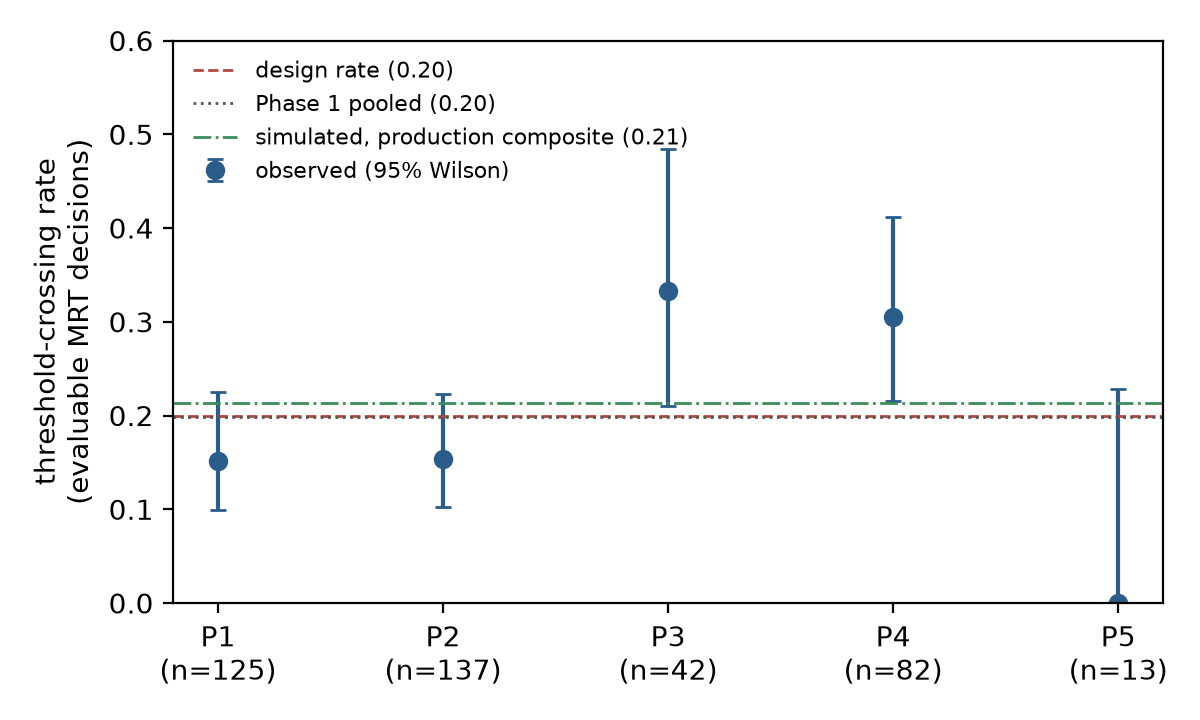
\includegraphics[width=0.75\textwidth]{field_check_crossing.png}
    \caption{Threshold-crossing rate per Phase 1 participant (95\% Wilson intervals) against the design rate of 0.20, the pooled Phase 1 rate, and the single-item and composite simulations. n: evaluable decisions from study day 7.}
\end{figure}

\section{Considerations for Future Deployments}

The following points are offered for future studies that use this engine. They are not changes proposed for REACT, which keeps the 80th-percentile expanding threshold and the protocol's stated detectable-effect range.

\begin{itemize}
    \item \textbf{A lower threshold percentile.} A 70th-percentile threshold would raise eligible decision points from 4.29 to 6.42 per participant per week in the single-item simulation (5.88 to 8.46 with the production composite), and with them availability. The cost is more crossings by low-volatility participants near the 1--7 scale's floor of about 0.33, where added prompts reflect rounding more than real change.
    \item \textbf{Power planning.} With availability near 0.21, each participant contributes roughly 20 to 35 randomized decision points (Paper B). A future trial with similar availability, fewer participants or lower engagement might plan its power around a minimum detectable effect of 0.20 to 0.25 rather than 0.10 to 0.15.
\end{itemize}

\end{document}
